% concatenated from CNAG20251031.tex
\documentclass[11pt]{amsart}
%\usepackage[left=1in,right=1in,top=1in,bottom=1in]{geometry}
\usepackage{color}

%\usepackage[all,cmtip]{xy}
%\usepackage{amssymb,mathtools}
%\usepackage[english]{babel}
%\usepackage{mathrsfs}
%

\usepackage{amsmath, amsfonts, amssymb, amsthm, faktor}

\usepackage[all]{xy}
\usepackage{tikz}
\usetikzlibrary{math}
\usetikzlibrary{patterns}
\usepackage{caption}
\usepackage{subfig}
\usepackage{cite}
%\usepackage{subcaption}
\usepackage{caption}
\usepackage{multirow}
\usetikzlibrary{arrows,chains,matrix,positioning,scopes,decorations.pathreplacing,
decorations.pathmorphing,decorations.markings,arrows.meta}

%\usepackage{chngcntr}
%\counterwithout{figure}{chapter}

\usepackage{aliascnt}
\usepackage[colorlinks, linktocpage, allcolors=black,breaklinks]{hyperref}

\usepackage{comment}
\usepackage{enumitem}






\newtheorem{theorem}{Theorem}[section]
\newtheorem{lemma}[theorem]{Lemma}

\newtheorem{proposition}[theorem]{Proposition}
\newtheorem{corollary}[theorem]{Corollary}

\theoremstyle{definition}
\newtheorem{definition}[theorem]{Definition}
\newtheorem{definitions}[theorem]{Definitions}
\newtheorem{example}[theorem]{Example}
\newtheorem{problem}[theorem]{Problem}
\newtheorem{problems}[theorem]{Problems}
\newtheorem{conjecture}[theorem]{Conjecture}
\newtheorem{conjectures}[theorem]{Conjectures}
\newtheorem{remark}[theorem]{Remark}
\newtheorem{remarks}[theorem]{Remarks}
\newtheorem{question}[theorem]{Question}
\newtheorem{questions}[theorem]{Questions}
\newtheorem{notation}[theorem]{Notation}
\newtheorem{fact}[theorem]{Fact}
\newtheorem{claim}{Claim}
\newtheorem{subclaim}{Subclaim}
\newtheorem{convention}[theorem]{Convention}
%%Macros
\def\triang#1{\bar{#1}}

\def\U{\mathbb{U}} %Urysohn space
\def\H{\mathbb{H}} 

\DeclareMathOperator{\dist}{Dist}
%\def\diam{\mathrm{Diam}}
\DeclareMathOperator{\diam}{diam}
\DeclareMathOperator{\lcm}{lcm}
%\def\Iso{\mathrm{Iso}}
\DeclareMathOperator{\Iso}{Iso}
%\def\Aut{\mathrm{Aut}}
\DeclareMathOperator{\Aut}{Aut}
\DeclareMathOperator{\Sym}{Sym}

\def\PSLS{partial strong L\'evy system}



\def\CDVS{countable distance value set}
\def\P{\mathcal{P}} %Partial isometries
\def\rng{\mathrm{rng}} %Range
\def\dom{\mathrm{dom}} %Domain
\def\setting{setting}
\def\settsymbol#1{\mathcal{#1}}
\def\map{\mathrm{MAP}}
\def\minap{\mathrm{MinAP}}
\newcommand{\sh}{\mbox{-}}
\newcommand{\Q}{\mathbb{Q}}
\newcommand{\Lan}{\mathcal{L}}
\newcommand{\M}{\mathcal{M}}
\newcommand{\NN}{\mathcal{N}}
\newcommand{\K}{\mathcal{K}}
%\newcommand{\M}{\mathbb{M}}
\newcommand{\A}{\mathcal{A}}
\newcommand{\B}{\mathcal{B}}
\newcommand{\C}{\mathcal{C}}
\newcommand{\R}{\mathcal{R}}
%-------------------


%------------------- Revision environments
%Our environment colors

\usepackage{color}
\newenvironment{revvy}{\color{magenta}}{}
\newenvironment{revdw}{\color{blue}}{}
\newenvironment{revsg}{\color{red}}{}

%------------------- Environment for Hugo's color
\def\by{\begin{revvy}}
\def\ey{\end{revvy}}
%-------------------
%------------------- Environment for David's color
\def\bd{\begin{revdw}}
\def\ed{\end{revdw}}
%-------------------
%------------------- Environment for Prof. Gao's color
\def\bg{\begin{revsg}}
\def\eg{\end{revsg}}
%-------------------

\def\N{\mathbb{N}} %Natural numbers
\def\Z{\mathbb{Z}}
\def\R{\mathbb{R}}
\def\T{\mathbb{T}}
\def\V{\mathcal{V}}
\def\C{\mathcal{C}}


\def\Ps#1{\mathbf{Ps}{(#1)}}

\def\cf{\mathrm{cf}}

\def\Cyc{\mathrm{Cyc}}
\def\grp#1{\langle{#1}\rangle}
\def\ssgp{$\mathrm{SSGP}$}
\def\Prm{\mathbf{P}}
\def\Z{\mathbb{Z}}
\def\Q{\mathbb{Q}}

\def\F{\mathbb{F}}
\def\a{m}
\def\bsft{\mathfrak{b}}

\def\dash#1{\bar{#1}}

\def\Oplus{+}

\def\wprod{*}
\def\fprod{\cdot}

\def\e#1{e}

\def\inv{\leftarrow}

\begin{document}
\title{Borel combinatorics of Schreier graphs of $\Z$-actions}



\author{Su Gao}
\address{School of Mathematical Sciences and LPMC, Nankai University, Tianjin 300071, P.R. China}
\email{sgao@nankai.edu.cn}

\author{Yingying Jiang}
\address{School of Mathematical Sciences and LPMC, Nankai University, Tianjin 300071, P.R. China}
\email{yyjiangmath@mail.nankai.edu.cn}

\author{Tianhao Wang}
\address{School of Mathematical Sciences and LPMC, Nankai University, Tianjin 300071, P.R. China}
\email{tianhao\_wang@qq.com}


\begin{abstract} In this paper we consider the Borel combinatorics of Schreier graphs of $\Z$-actions with arbitrary finite generating sets. We formulate the Borel combinatorics in terms of existence of Borel equivariant maps from $F(2^\Z)$ to subshifts of finite type. We then show that the Borel combinatorics and the continuous combinatorics coincide, and both are decidable. This is in contrast with the case of $\Z^2$-actions. We then turn to the problem of computing Borel chromatic numbers for such graphs. We give an algorithm for this problem which runs in exponential time. We then prove some bounds for the Borel chromatic numbers and give a formula for the case where the generating set has size $4$.
\end{abstract}

%\subjclass[2010]{Primary: 22A05; Secondary: 03E99, 06A06, 20E05, 54E35, 54H11}

%\keywords{topologically simple group, free group, minimally almost periodic group, small subgroup generating property}

\maketitle
%\tableofcontents

\section{Introduction}
Borel combinatorics studies combinatorial properties of topological graphs or more generally Borel graphs. Since the seminal paper of Kechris, Solecki and Todorcevic \cite{KST} on Borel chromatic numbers, many researchers have contributed to this new and rapidly growing area of research; a comprehensive survey can be found in the recent book by Kechris and Marks \cite{KM}.

One of the reasons Borel combinatorics is interesting to researchers is that one obtains different answers to combinatorial questions when imposing definability requirements on the combinatorial objects. For instance, Laczkovich realized early on that the graph on the unit circle defined by a rotation by a fixed irrational angle has chromatic number $2$ (since every connected component is isomorphic to a bi-infinite path) but its Borel chromatic number is necessarily $3$, that is, any set of colors one needs to use to find a Borel proper coloring function from this graph must have at least $3$ elements. 

More recently, it was discovered by Gao, Jackson, Krohne and Seward \cite{GJKS, GJKS2} that there is a further difference between Borel combinatorics and continuous combinatorics for topological graphs for nontrivial reasons. For instance, the above graph considered by Laszkovich does not have a sensible continuous chromatic number because the space is connected. But if one considers the space with one connected component removed, then it becomes zero-dimensional and the continuous chromatic number makes sense and can be seen to be $3$ (while the Borel chromatic number remains $3$). Answering a question of \cite{KST}, the authors of \cite{GJKS2} considered the free part of the $\Z^2$-action on the shift space $2^{\Z^2}$, and showed that the Borel chromatic number is $3$; in contrast, they also showed  (see \cite{GJKS}) that the continuous chromatic number is $4$. A similar difference exists for edge chromatic numbers of this graph (see \cite{BHT, CU, GJKS, GWW, GR, Weil}).

The computations of chromatic numbers and edge chromatic numbers belong to a class of questions known as {\em locally checkable labelling} (\emph{LCL}) problems (see, e.g., \cite{GR, GR2}), a concept that had been studied in distributed computing in computer science (see, e.g. \cite{BHKetc}). Bernshteyn's influential work \cite{Ber} connected the distributed computing and Borel combinatorics together. There are now many results that characterize the descriptive-set-theoretic complexity of LCL problems by the computational complexity of local algorithms that solve the problem in a distributed fashion. 

In this paper we study the Borel chromatic numbers of Schreier graphs that come from $\Z$-actions but with arbitrary finite sets of generators. More generally, we formulate the LCL problems in terms of the existence of Borel equivariant maps from $F(2^\Z)$, the free part of the $\Z$-action on the shift space $2^\Z$, to certain subshifts of finite type. Then we show that the Borel combinatorics in this context is the same as the continuous combinatorics, via the following main theorem.

\begin{theorem}\label{thm:1.1} Let $X$ be a $\Z$-subshift of finite type. Then the following are equivalent:
\begin{enumerate}
\item[\rm (1)] There exists a Borel equivariant map from $F(2^\Z)$ to $X$;
\item[\rm (2)] There exists a continuous equivariant map from $F(2^\Z)$ to $X$.
\end{enumerate}
\end{theorem}

By the results of \cite{GJKS, GJKS2}, we know that the theorem fails when $\Z$ is replaced by $\Z^2$. In fact, using some results of \cite{GJKS} we give a more concrete characterization of the above problems, and show that the problem is actually decidable, that is, there is an algorithm which, given a subshift of finite type, computes whether there exists a Borel equivariant map from $F(2^\Z)$ to $X$.

We then apply the main theorem to the problem of computing Borel chromatic numbers. If $S$ is a finite generating set of $\Z$ that is symmetric (i.e., $S=-S$) and $0\not\in S$, we obtain a Schreier graph $G_S$ on $F(2^\Z)$ by putting an edge between $x$ and $y$ if and only if there is $s\in S$ such that $s\cdot x=y$. As mentioned above, this problem is now computable, that is, given $S$, the Borel chromatic number of $G_S$ is a computable function with $S$ as input. However, the naive algorithm that computes the Borel chromatic number takes exponential time in $\max S$. Thus it is still not feasible for us to compute the full answer of this problem. 

We then prove some partial results on this problem. Specifically, we prove some results on the upper and lower bounds, and then obtain the exact answers in some special cases. The following are our main results.

\begin{theorem}\label{thm:1.2} Let $S=\{\pm a_1,\dots, \pm a_n\}$ with $\gcd(a_1,\dots, a_n)=1$. Let $\chi(S)$ be the Borel chromatic number of $G_S$. Then the following hold.
\begin{enumerate}
\item[\rm (1)] $3\leq \chi(S)\leq \left\lfloor\displaystyle\frac{3}{2}n\right\rfloor +1$.
\item[\rm (2)] If $S\cap (k+1)\Z=\varnothing$ for some $k\geq 1$, then $\chi(S)\leq k+2$.
\item[\rm (3)] If $(a_1,\dots, a_n)=(1,\dots, n)$, then $\chi(S)=n+2$.
\item[\rm (4)] If $n=2$ and $(a_1, a_2)\neq (1,2)$, then $\chi(S)=3$.
\end{enumerate}
\end{theorem}

We are not able to give a general formula for $\chi(S)$ when $n\geq 3$, but our method can determine the value of $\chi(S)$ for many different types of $S$. In particular, we show that for any $n\geq 1$ and $3\leq k\leq n+2$, there is a generating set $S$ as above where $|S|=2n$ and $\chi(S)=k$. However, we do not have any example of an $S$ where $|S|=2n$ but $\chi(S)>n+2$.

The rest of the paper is organized as follows. In Section~\ref{sec:2} we recall some preliminary concepts and results in descriptive set theory, topological dynamics, and graph theory. In particular, we explain how to formulate Borel combinatorics by the existence of Borel equivariant maps into subshifts of finite type. In Section~\ref{sec:3} we prove Theorem~\ref{thm:1.1} and give a finitary characterization which is equivalent to both clauses of Theorem~\ref{thm:1.1}. This finitary characterization turns out to be decidable. Starting from Section~\ref{sec:4} we turn to the problem of finding Borel chromatic numbers of $G_S$. In Section~\ref{sec:4} we give an algorithm for the problem. However, the algorithm runs in exponential time in $\max S$. In Section 5 we prove Theorem~\ref{thm:1.2} (1)--(3) and give some conseqences. In Section 6 we prove Theorem~\ref{thm:1.2} (4). Finally, in Section 7 we make some remarks about the case $|S|=6$.

\section{Preliminaries}\label{sec:2}

In this section we recall some preliminary concepts and results in descriptive set theory, topological dynamics, and graph theory. 

A topological space $X$ is {\em Polish} if it is separable and completely metrizable. If $X$ is a Polish space and $Y\subseteq X$, then the subspace topology on $Y$ is Polish if and only if $Y$ is a $G_\delta$ subset in $X$, i.e., $Y$ is the intersection of countably many open subsets of $X$. The collection of all {\em Borel sets} in a Polish space $X$ is the smallest $\sigma$-algebra generated by the collection of all open subsets of $X$. If $X, Y$ are Polish spaces, then $f\colon X\to Y$ is {\em continuous} if for any open subset $U\subseteq Y$, $f^{-1}(U)$ is an open subset of $X$, and $f$ is {\em Borel-measurable}, or simply {\em Borel}, if for any open subset $U\subseteq Y$, $f^{-1}(U)$ is a Borel subset of $X$.

Let $X$ be a Polish space and $A\subseteq X$. We say that $A$ is {\em comeager} if $A$ contains a dense $G_\delta$ subset of $X$. By definition, a comeager set is dense. By the Baire category theorem, in a Polish space the intersection of countably many comeager sets is still comeager. If $Y$ is another Polish space and $f\colon X\to Y$ is Borel, then there is a comeager $C\subseteq X$ such that $f\upharpoonright C\colon C\to Y$ is continuous.

We consider the shift space $\bsft^\Z=\{0,\dots,\bsft-1\}^\Z$ for some $\bsft\geq 1$. For $s\in \Z$ and $y\in \bsft$, the $\Z$-action is defined by the shift map
$$ (s\cdot y)(n)=y(n+s) $$
for any $n\in\Z$.  We equip $\bsft$ with the discrete topology, and $\bsft^\Z$ with the product topology. With this topology, $\bsft^\Z$ is a compact Polish space and the shift map is continuous. For any $y\in \bsft^Z$, the {\em orbit} of $y$ is 
$$ [y]=\left\{s\cdot y\colon s\in \Z\right\}. $$
A subset $Y$ of $\bsft^\Z$ is {\em shift-invariant} if for any $y\in Y$, we have $[y]\subseteq Y$. A closed shift-invariant subset of $\bsft^\Z$ is called a {\em subshift} of $\bsft^\Z$. 

In this context, a {\em pattern} $p$ is a nonempty finite word in the alphabet $\mathfrak{b}$. We regard a pattern $p$ as a function from $\{0, \dots, \ell(p)-1\}$ to $\{0,\dots, \bsft-1\}$, where $\ell(p)\geq 1$ is the {\em length} of $p$. If $y\in \bsft^\Z$ and $p$ is a pattern, then we say that $p$ {\em occurs} in $y$ if there is $n\in\Z$ such that for any $0\leq i<\ell(p)$, $p(i)=y(n+i)$; otherwise $p$ {\em does not occur} in $y$. 

Given patterns $p_1, \dots, p_k$, define a subshift 
$$ Y=Y_{(\bsft; p_1,\dots,p_k)}=\left\{y\in \bsft^\Z\colon \mbox{none of $p_1,\dots, p_k$ occur in $y$}\right\}. $$
$Y$ is a closed shift-invariant subset of $\bsft^\Z$, hence a subshift. Here $Y$ is called the {\em subshift of finite type} described by $(\bsft; p_1,\dots, p_k)$, and the patterns $p_1,\dots, p_k$ in the description of $Y$ are called the {\em forbidden patterns}. Any subshift of finite type can be equivalently described by forbidden patterns of the same length. Thus, in our discussions, we tacitly assume that the forbidden patterns have the same length.

The {\em free part} of $\bsft^\Z$ is
$$ F(\bsft^\Z)=\left\{y\in \bsft^\Z\colon \mbox{for any nonzero $s\in \Z$, $s\cdot y\neq y$}\right\}. $$
$F(\bsft^\Z)$ is a shift-invariant subset of $\bsft^\Z$. However, it is not closed, but a $G_\delta$ subset, hence it is a Polish space (and it is no longer compact). In this paper, we only consider $F(2^\Z)$, the free part of $2^\Z$.

A map $f\colon F(2^\Z)\to Y$, where $Y$ is a subshift of $\bsft^\Z$, is {\em equivariant} if for any $s\in \Z$ and $x\in F(2^\Z)$, we have $f(s\cdot x)=s\cdot f(x)$. 

Let $S$ be a finite generating set for $\Z$, i.e., $\langle S\rangle=\Z$. We tacitly assume that $0\not\in S$ and $S$ is {\em symmetric}, i.e., $S=-S$. The {\em Cayley graph} $C_S$ is the graph $(\Z, E_S)$, where $uv\in E_S$ exactly when $u-v\in S$. The {\em Schreier graph} $G_S$ is the graph $(2^\Z, W_S)$, where $xy\in W_S$ exactly when there is $s\in S$ such that $s\cdot x=y$. No matter what the generating set $S$ is, the connected components of $G_S$ are exactly the orbits of $2^\Z$. Thus it makes sense to speak of the Schreier graph on a shift-invariant subset of $2^\Z$, such as $F(2^\Z)$. Note that because of the freeness, each connected component of $F(2^\Z)$ is isomorphic to the Cayley graph $C_S$. 

In general, if $K$ is a set and $G=(V,E)$ is a graph, a {\em proper $K$-coloring} of $G$ is a function $c\colon V\to K$ for some some set $K$ such that whenever $uv\in E$, we have $c(u)\neq c(v)$. The {\em chromatic number} of $G$ is the least cardinality of $K$ such that there exists a proper $K$-coloring of $G$. When $G$ is a topological graph, as in the case of $G_S$ defined above, we may equip the set $K$ with the discrete topology and consider proper $K$-coloring functions from $G$ to $K$ that are continuous or Borel, and then define the corresponding notions of {\em continuous chromatic number} or {\em Borel chromatic number} of $G$. For all of the graphs we consider in this paper, all of the different versions of the chromatic numbers are finite.



Now, LCL problems on $G_S$ can be reformulated in terms of equivariant maps from $F(2^\Z)$ to some suitably defined subshifts of finite type. Here we will not define LCL problems in general, but give only an example of how the existence of a proper $\bsft$-coloring of $G_S$ corresponds to an equivariant map from $F(2^\Z)$ to a subshift of $\bsft^\Z$ of finite type. Let $\ell=\max S+1$. We define a finite set $F$ of forbidden patterns of length $\ell$ in the alphabet $\bsft$  by
$$ p\in F\iff \exists 0\leq i<\ell\ \exists s\in S\ (0\leq i+s<\ell \mbox{ and } p(i)=p(i+s)). $$
Enumerate $F$ as $p_1,\dots, p_k$. Then it is straightforward to check by definition that the following are equivalent:
\begin{enumerate}
\item[(1)] There exists an equivariant map $f\colon F(2^\Z)\to Y_{(\bsft; p_1, \dots, p_k)}$;
\item[(2)] There exists a proper $\bsft$-coloring of $G_S$.
\end{enumerate}
Additionally, if we enhance both (1) and (2) by requiring the maps (or the coloring functions) to be continuous or Borel, the enhanced versions are still equivalent. 

Thus, in this paper, by the {\em continuous} (or {\em Borel}) {\em combinatorics} of $F(2^\Z)$, we mean the problem of the existence of a continuous (or Borel, respectively) equivariant map from $F(2^\Z)$ to an arbitrary subshift of finite type.

\section{Borel combinatorics versus continuous combinatorics}\label{sec:3}

A characterization of the continuous combinatorics of $F(2^\Z)$ has already been given in \cite[Section 2.2]{GJKS}, where the main theorem \cite[Theorem 2.2.2]{GJKS} has been dubbed the Two-Tiles Theorem (we will recall the details below). Here we expand this characterization and show that the Borel combinatorics and the continuous combinatorics coincide. 

To state our main result we need to first recall some definitions from \cite[Section 2.2]{GJKS}. 

We first define an infinite family of finite directed graphs 
$$\left\{\Gamma_{n,p,q}\colon 1\leq n\leq p, q\right\},$$ 
which we call {\em two-tiles graphs}. For any integers $a, b$ with $1\leq a\leq b$, let $T(a,b)$ be a simple directed path of length $a+b-1$. Note that $T(a, b)$ consists of $a+b$ many vertices and $a+b-1$ many edges. When enumerating the vertices of $T(a,b)$, we always start with the unique vertex with $0$ indegree and follow the directions of the edges. With this convention we may speak of the first $n$ vertices, the last $n$ vertices, etc. Now, to define $\Gamma_{n,p,q}$ we fix $1\leq n\leq p, q$. Let $T_1(n, p, q)$ be a copy of $T(n,p)$ and let $T_2(n,p,q)$ be a copy of $T(n,q)$. Then let $\Gamma_{n,p,q}$ be the directed graph obtained from first taking the disjoint union of $T_1(n,p,q)$ and $T_2(n,p,q)$ and then identifying the following four subgraphs of $T_1(n,p, q)$ and $T_2(n,p,q)$:
\begin{itemize}
\item the subgraph of $T_1(n,p,q)$ induced by its first $n$ vertices,
\item the subgraph of $T_1(n,p,q)$ induced by its last $n$ vertices,
\item the subgraph of $T_2(n,p,q)$ induced by its first $n$ vertices, and
\item the subgraph of $T_2(n,p,q)$ induced by its last $n$ vertices.
\end{itemize}
Note that each of these subgraphs is a simple directed path of length $n-1$, and there is a unique isomorphism between any two of these subgraphs. Hence there is a unique way to implement the identification step of the construction. Figure~\ref{fig:onedimgamma} illustrates the graphs $T_1(3,7,9)$, $T_2(3,7,9)$ and $\Gamma_{3,7,9}$.

\begin{figure}[h]
\centering
\subfloat
{
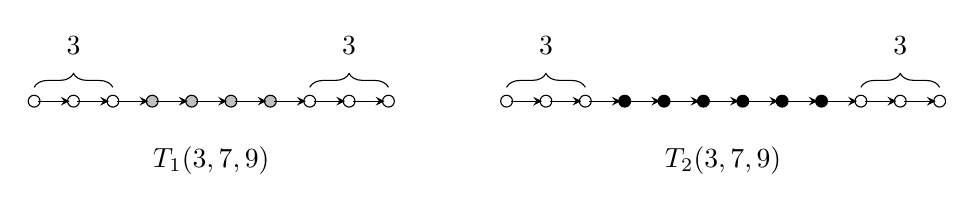
\begin{tikzpicture}[scale=0.5]
\pgfmathsetmacro{\n}{3}
\pgfmathsetmacro{\p}{7}
\pgfmathsetmacro{\q}{9}
\pgfmathsetmacro{\a}{-7}
\pgfmathsetmacro{\b}{5}
\pgfmathsetmacro{\d}{4.5}
\pgfmathsetmacro{\e}{5.5}
\pgfmathsetmacro{\x}{\n+\p+\n-1}
\pgfmathsetmacro{\y}{\n+\q+\n-1}
\pgfmathsetmacro{\xa}{\n+\p-2}
\pgfmathsetmacro{\ya}{\n+\q-2}
\pgfmathsetmacro{\nm}{\n-1}
\pgfmathsetmacro{\pm}{\p-\n-1}
\pgfmathsetmacro{\qm}{\q-\n-1}
\foreach \i in {0,...,\nm}
{ \draw (\a+\i,0) circle (0.15);
}
\foreach \i in {0,...,\pm}
{ \draw[fill=lightgray] (\a+\n+\i,0) circle (0.15);
}
\foreach \i in {0,...,\nm}
{ \draw  (\a+\p+\i,0) circle (0.15);
}
\foreach \i in {0,...,\xa}
{ \draw[->,>=stealth] (\a+\i+0.1,0) -- (\a+\i+0.9,0);
}


\foreach \i in {0,...,\nm}
{ \draw  (\b+\i,0) circle (0.15);
}
\foreach \i in {0,...,\qm}
{ \draw[fill=black] (\b+\n+\i,0) circle (0.15);
}
\foreach \i in {0,...,\nm}
{ \draw  (\b+\q+\i,0) circle (0.15);
}
\foreach \i in {0,...,\ya}
{ \draw[->,>=stealth] (\b+\i+0.1,0) -- (\b+\i+0.9,0);
}

\draw[decorate, decoration={brace, mirror, amplitude=5pt},yshift=10pt] (\a+\n-1,0) -- (\a,0)
node [black,midway,yshift=15pt] {$3$};

\node at (\a+\d, -1.5) {$T_1(3,7,9)$};

\draw[decorate, decoration={brace, mirror, amplitude=5pt},yshift=10pt] (\a+\p+\n-1,0) -- (\a+\p,0)
node [black,midway,yshift=15pt] {$3$};

\draw[decorate, decoration={brace, mirror, amplitude=5pt},yshift=10pt] (\b+\n-1,0) -- (\b,0)
node [black,midway,yshift=15pt] {$3$};

\node at (\b+\e,-1.5) {$T_2(3,7,9)$};

\draw[decorate, decoration={brace, mirror, amplitude=5pt},yshift=10pt] (\b+\q+\n-1,0) -- (\b+\q,0)
node [black,midway,yshift=15pt] {$3$};

\end{tikzpicture}
}
\vspace{5pt}
\subfloat
{
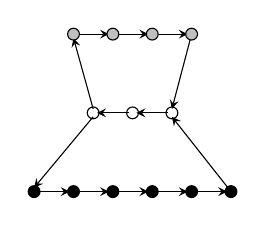
\begin{tikzpicture}[scale=0.5]
\pgfmathsetmacro{\n}{3}
\pgfmathsetmacro{\p}{7}
\pgfmathsetmacro{\q}{9}
\pgfmathsetmacro{\a}{-10}
\pgfmathsetmacro{\b}{5}

\pgfmathsetmacro{\c}{-0.5}
\pgfmathsetmacro{\d}{2}
\pgfmathsetmacro{\e}{\p-\n-1}
\pgfmathsetmacro{\em}{\e-1}
\pgfmathsetmacro{\h}{0.1}

\pgfmathsetmacro{\f}{\q-\n-1}
\pgfmathsetmacro{\fm}{\q-\n-2}

\pgfmathsetmacro{\x}{\n+\p+\n-1}
\pgfmathsetmacro{\y}{\n+\q+\n-1}
\pgfmathsetmacro{\nm}{\n-1}
\pgfmathsetmacro{\nmm}{\n-2}
\pgfmathsetmacro{\pm}{\p-1}
\pgfmathsetmacro{\qm}{\q-1}

\foreach \i in {0,...,\em}
{ \draw[->,>=stealth] (\a+\c+\i+0.1,\d) -- (\a+\c+\i+0.9,\d);
}

\foreach \i in {0,...,\nmm}
{ \draw[->,>=stealth] (\a+\i+0.9,0) -- (\a+\i+0.1,0);
}

\foreach \i in {0,...,\fm}
{ \draw[->,>=stealth] (\a-1.5+\i+0.1,-\d) --  (\a-1.5+\i+0.9,-\d);
}

\draw[->,>=stealth]  (\a,\h) -- (\a+\c,\d-\h);
\draw[->,>=stealth] (\a+\c+\e,\d) -- (\a+\nm,\h);
\draw[->,>=stealth] (\a,-\h) -- (\a-1.5,-\d+\h);
\draw[->,>=stealth]  (\a-1.5+\f,-\d) -- (\a+\nm,-\h);

\foreach \i in {0,...,\e}
{ \draw[fill=lightgray] (\a+\c+\i,\d) circle (0.15);
}

\foreach \i in {0,...,\nm}
{ \draw (\a+\i,0) circle (0.15);
}

\foreach \i in {0,...,\f}
{ \draw[fill=black] (\a-1.5+\i,-\d) circle (0.15);
}

\end{tikzpicture}
}
\caption{\label{fig:onedimgamma}The construction of the two-tiles graph $\Gamma_{3,7,9}$.
}
\end{figure}

\begin{definition} Let $Y\subseteq \bsft^\Z$ be a subshift of finite type described by the sequence
$(\bsft;p_1,\dots,p_k)$ and let $g \colon \Gamma_{n,p,q}
\to \bsft$ be a map. We say that $g$  {\em respects} $Y$ if for any $1\leq i\leq k$ and for any directed path $v_1\cdots v_{\ell(p_i)}$ of length $\ell(p_i)-1$ in $\Gamma_{n,p,q}$, the word $g(v_1)\cdots g(v_{\ell(p_i)})$ of length $\ell(p_i)$ in alphabet $\bsft$ is not equal to $p_i$.
\end{definition}

The following is our main theorem of this section.

\begin{theorem} \label{thm:main}
Let $Y$ be the subshift of finite type described by $(\bsft; p_1,\dots, p_k)$. Then the following are equivalent.
\begin{enumerate}[label=\rm{(\arabic*)}, ref=\arabic*]
\item\label{odd}
There is a Borel equivariant map from $F(2^\Z)$ to $Y$.
\item\label{oda}
There is a continuous equivariant map from $F(2^\Z)$ to $Y$.
\item\label{odb}
There are integers $n,p,q$ with $\ell(p_1)\leq n<p,q$ and $\gcd(p,q)=1$, and there is $g \colon \Gamma_{n,p,q}\to \bsft$ which respects $Y$.
\item\label{odc}
For all $n\geq \ell(p_1)$ and for all sufficiently large $p,q>n$,
 there is $g \colon  \Gamma_{n,p,q}\to \bsft$ which respects $Y$.
\end{enumerate}
\end{theorem}

\begin{proof} The equivalence of (\ref{oda})--(\ref{odc}) is the Two-Tiles Theorem \cite[Theorem 2.2.2]{GJKS}. It is clear that (\ref{oda}) implies (\ref{odd}). It suffices to prove (\ref{odd}) implies (\ref{odc}).

Let $f\colon F(2^\Z)\to Y$ be a Borel equivariant map. There is a comeager set $C\subseteq F(2^\Z)$ so that $f\upharpoonright C\colon C\to Y$ is continuous. Let $D=\bigcap_{n\in\Z} n\cdot C$. Then $D$ is still comeager and $f\upharpoonright D\colon D\to Y$ is still continuous. Arbitrarily fix $x_0\in D$ and $n\geq \ell(p_1)$. The set
$$ U=\{ y\in \bsft^\Z\colon y(i)=f(x_0)(i) \mbox{ for all $0\leq i<n$}\} $$
is a basic open set in $Y$, and $x_0\in f^{-1}(U)\cap D$. By the continuity of $f\upharpoonright D$ on $D$, there is a basic open set $V$ of $F(2^\Z)$ such that $x_0\in V\cap D\subseteq f^{-1}(U)\cap D$. Without loss of generality, we may assume 
$$ V=\{z\in F(2^\Z)\colon z(i)=x_0(i) \mbox{ for all $a\leq i\leq b$}\} $$
for some $a<b\in \Z$. Now let $p, q>\max\{b-a, n\}$ be such that $\gcd(p,q)=1$. Then
$$ W=(-p\cdot V)\cap V\cap (q\cdot V) $$
is a nonempty open set in $F(2^\Z)$, and thus $W\cap D\neq\varnothing$ since $D$ is comeager. Now let $x\in W\cap D$ and $y=f(x)$. Then $x\in V\cap D$, and therefore $y\in U$. We also have $p\cdot x\in V\cap p\cdot D=V\cap D$ and therefore $$p\cdot y=p\cdot f(x)=f(p\cdot x)\in U. $$
Similarly, $-q\cdot x\in V\cap D$ and $-q\cdot y\in U$.

We now regard the Cayley graph of $\Z$ between $a-p$ and $b$ as $T_1(n,p,q)$ and between $a$ and $b+q$ as $T_2(n,p,q)$. Define $g\colon T_1(n, p,q)\to \bsft$ by $g(i)=y(i)$ for $a-p\leq i\leq b$, and define
$g\colon T_2(n,p,q)\to \bsft$ also by $g(i)=y(i)$ for $a\leq i\leq b+q$. It is easily seen that the values of $g$ for the first $n$ and last $n$ vertices of $T_1(n,p,q)$ and $T_2(n,p,q)$ coincide, and therefore this definition naturally induces a map $g\colon \Gamma_{n,p,q}\to \bsft$ which is well defined. Moreover, suppose $1\leq i\leq k$ and $v_1\dots v_{\ell(p_i)}$ is a directed path in $\Gamma_{n,p,q}$, then it is entirely contained in either $T_1(n,p,q)$ or $T_2(n,p,q)$. Thus $g(v_1)\dots g(v_{\ell(p_i)})$ is a word which occurs in $y$. Since $y\in Y$, we conclude that $g(v_1)\dots g(v_{\ell(p_i)})$ cannot be equal to $p_i$. This shows that $g$ respects $Y$. 
\end{proof}

Since it has been shown in \cite[Theorem 4.2.1]{GJKS} that the continuous combinatorics is decidable, we have the following immediate corollary.

\begin{corollary}\label{cor:decidable} The Borel combinatorics of $F(2^\Z)$ is decidable. That is, the set of parameters $(\bsft; p_1,\dots, p_k)$ for which there exists a Borel equivariant map from $F(2^\Z)$ to $Y_{(\bsft; p_1,\dots, p_k)}$ is decidable.
\end{corollary}
























\section{An algorithm for Borel chromatic numbers}\label{sec:4}

In the rest of this paper, we focus on the problem of computation of Borel chromatic numbers of the Schreier graphs $G_S$ for finite generating sets of $\Z$. We will present a generating set $S$ by the enumeration of its positive members in increasing order. We introduce the following notation.

\begin{definition} Denote by $\Sigma$ the set of all strictly increasing sequence of positive integers $a_1<\dots<a_n$ such that $\gcd(a_1,\dots, a_n)=1$. For $(a_1,\dots, a_n)\in \Sigma$, denote by $\chi(a_1,\dots, a_n)$ the Borel chromatic number of the Schreier graph $G_S$, where $S=\{\pm a_1,\dots, \pm a_n\}$. 
\end{definition}

We will show in the next section that for any $(a_1,\dots, a_n)\in \Sigma$, 
$$ 3\leq \chi(a_1,\dots, a_n)\leq 2n. $$
By Corollary~\ref{cor:decidable}, $\chi$ is a computable function. In fact, given $(a_1,\dots, a_n)\in\Sigma$, to compute $\chi(a_1,\dots, a_n)$ it suffices to successively check if there is a Borel proper $\bsft$-coloring for $\bsft=3, \dots, 2n$, until a postive answer is found; the smallest such $\bsft$ is $\chi(a_1,\dots, a_n)$.

In the following we describe an algorithm {\tt BPC} for checking whether there is a Borel proper coloring.


{\tt Input:} A sequence $(a_1,\dots, a_n)\in \Sigma$ and an integer $\bsft\in [3, 2n]$.

{\tt Step 1:} Let $m=a_n+1$ and let $\bsft^m$ be the set of all words of length $m$ in the alphabet $\bsft$. Form the set
$$ V=\left\{ u\in \bsft^m\colon u(j)\neq u(j+a_i) \mbox{ for all $1\leq i\leq n$ and $0\leq j\leq a_n-a_i$}\right\}. $$
Construct a directed graph $H=(V, E)$, where
$$ uv\in E\iff \mbox{ for all $0\leq j<m$, $v(j)=u(j+1)$.} $$

{\tt Step 2:} For each connected component $C$ of $H$, compute the  value of the following function $f$:
$f(C)=\infty$, if there are no directed cycles in $C$; otherwise, $f(C)=\mbox{the $\gcd$ of the lengths of all directed cycles}$. 
 If for some connected component $C$ of $H$, $f(C)=1$, then return and output {\tt yes}. Otherwise, output {\tt no}.

This finishes the algorithm {\tt BPC}.

The correctness of the algorithm {\tt BPC} follows from the proof of \cite[Theorem 4.2.1]{GJKS}. The value in {\tt Step 2} is known as the {\em period} of the directed graph, or when the graph is represented by its adjacency matrix, the {\em period} of the matrix. It is well studied in algebraic graph theory, symbolic dynamics and matrix theory (see, e.g., \cite[Section 4.5]{LindBook} and \cite[Section 8.5]{HornBook}). There are well-known algorithms for {\tt Step 2} which runs in $O(N^3)$ time for directed graphs with $N$ vertices (for instance, this follows from Wielandt's theorem \cite[Corollary 8.5.8]{HornBook} on the primitivity of nonnegative matrices). However, the only upper bound we know for the size of a connected component of $H$ is $\bsft^m$. Thus {\tt BPC} runs in time which is exponential in $\max S$.
































\section{Some bounds for Borel chromatic numbers}\label{sec:5}

In this section we prove some results that provide lower and upper bounds for the function $\chi(a_1,\dots, a_n)$. In some cases they give the correct values of $\chi$.

We will use the following notion in our proofs. We regard any finite simple directed path $T$ as an interval in $\Z$ with $xy\in T$ if and only if $x+1=y$. Thus we have an order on $T$ and can perform basic arithmetic operations on the vertices of $T$. Similarly for infinite or bi-infinite simple directed paths. Recall that for integers $a, b$ with $1\leq a\leq b$, $T(a, b)$ is the simple directed path of length $a+b-1$. We let $T(a, b)^{-}$ denote the subgraph of $T(a, b)$ induced by its first $a$ vertices, and $T(a, b)^+$ denote the subgraph of $T(a, b)$ induced by its last $a$ vertices.

\begin{definition} Let $S=\{\pm a_1,\dots, \pm a_n\}$ be a generating set of $\Z$ with $(a_1,\dots, a_n)\in \Sigma$. Let $G$ be a finite or infinite simple directed path. Let $\bsft\geq 1$ be an integer. An {\em $S$-coloration} of $G$ {\em with $\bsft$ colors} is a function $c\colon G\to \bsft$ such that for any $x, y\in G$, $c(x)\neq c(y)$ whenever $x-y\in S$. 
\end{definition}

The following lemma is an immediate corollary of Theorem~\ref{thm:main} and is our basic tool in the study of the function $\chi$. 

\begin{lemma}\label{lem:basic} For any generating set $S=\{\pm a_1,\dots, \pm a_n\}$ with $(a_1,\dots, a_n)\in \Sigma$, and for any integer $k\geq 1$, the following hold.
\begin{enumerate}
\item[\rm (a)] $\chi(a_1,\dots, a_n)>k$ if and only if for some $\ell\geq a_n+1$, there are arbitrarily large $p, q>\ell$ with $\gcd(p, q)=1$
such that there are no $S$-colorations $c_1$ of $T_1(\ell, p, q)$ and $c_2$ of $T_2(\ell, p, q)$ with $k$ colors such that the $c_1$ and $c_2$ agree on the subgraphs $T_1(\ell, p, q)^{\pm}$ and $T_2(\ell, p, q)^{\pm}$.
\item[\rm (b)] $\chi(a_1,\dots, a_n)\leq k$ if and only if for some $\ell\geq a_n+1$, there are $p, q>\ell$ with $\gcd(p, q)=1$ and $S$-colorations $c_1$ of $T_1(\ell, p, q)$ and $c_2$ of $T_2(\ell, p, q)$ with $k$ colors such that the $c_1$ and $c_2$ agree on the subgraphs $T_1(\ell, p, q)^{\pm}$ and $T_2(\ell, p, q)^{\pm}$.
\end{enumerate}
\end{lemma}

Now we consider lower bounds. 

\begin{definition} Given a generating set $S=\{\pm a_1,\dots, \pm a_n\}$ with $(a_1,\dots, a_n)\in \Sigma$, let $K_S$ denote the subgraph of the Cayley graph $C_S$ induced by $\{0, a_1,\dots, a_n\}$, and call it the {\em core subgraph} of $G_S$. Denote by $\lambda_S$ the size of the largest clique in $K_S$, and by $\kappa_S$ the chromatic number of $K_S$.
\end{definition}

The following result gives some general lower bounds.

\begin{theorem}\label{thm:lower} For any generating set $S=\{\pm a_1,\dots, \pm a_n\}$ with $(a_1,\dots, a_n)\in \Sigma$, we have
$$\chi(a_1,\dots, a_n)\geq \kappa_S+1\geq \lambda_S+1\geq 3. $$
\end{theorem}

\begin{proof} It is clear that $\kappa_S\geq \lambda_S\geq 2$. It remains to show that $\chi(a_1,\dots, a_n)>\kappa_S$. Denote $\ell=a_n+1$ and $k=\kappa_S$. We will use Lemma~\ref{lem:basic} (a).

We first claim that for any $m\geq \ell$, an $S$-coloration $c$ of $T(\ell, m)$ with $k$ colors is determined by the restriction of $c$ on $T(\ell, m)^-$. This is to say, if $c, c'$ are both $S$-colorations of $T(\ell, m)$ with $k$ colors, and $c\upharpoonright T(\ell, m)^{-}=c'\upharpoonright T(\ell, m)^-$, then $c=c'$. For notational simplicity, identify $T(\ell, m)$ with the interval $[0, \ell+m)$ in $\Z$. To prove the claim, it suffices to show that $c(\ell)=c'(\ell)$; for the rest of the vertices in $T(\ell, m)$, the claim follows by an induction from left to right. Now consider the subgraph $X_S$ of the Cayley graph $C_S$ induced by $\{\ell, \ell-a_1, \dots, \ell-a_n\}$. $X_S$ is isomorphic to $K_S$ via the isomorphism $x\mapsto \ell-x$. Thus the chromatic number of $X_S$ is $k$. Let $Y=X_S\setminus \{\ell\}$. Then $Y\subseteq T(\ell, m)^-$. We note that $c(Y)$ contains exactly $k-1$ colors. This is because, if $|c(Y)|<k-1$, then any extension of $c$ to a proper coloring on $X_S=Y\cup \{\ell\}$ uses $<k$ colors, contradicting the fact that the chromatic number of $X_S$ is $k$. It follows that $c(\ell)$ is the only color not used in $c(Y)$. Similarly, $c'(\ell)$ is the only color not used in $c'(Y)$. Since $c(Y)=c'(Y)$, we have $c(\ell)=c'(\ell)$ as required. 

Now we are ready to prove $\chi(a_1,\dots, a_n)>k$. Toward a contradiction, assume this fails. Then by Lemma~\ref{lem:basic} (a), for sufficiently large $p, q>\ell$ with $\gcd(p, q)=1$, there are $S$-colorations $c_1$ of $T_1(\ell, p, q)$ and $c_2$ of $T_2(\ell, p, q)$ with $k$ colors such that $c_1$ and $c_2$ agree on $T_1(\ell, p, q)^{\pm}$ and $T_2(\ell, p, q)^{\pm}$. Let $p$ and $q=p+a_1$ be sufficiently large with $\gcd(p, q)=1$. Let $c_1$ and $c_2$ be given with the above property. Then by the above claim, $c_1$ is determined by $c_1\upharpoonright T_1(\ell, p, q)^-$ and $c_2$ is determined by $c_2\upharpoonright T_2(\ell, p, q)^{-}$. Since 
$$c_1\upharpoonright T_1(\ell, p, q)^-=c_2\upharpoonright T_2(\ell, p, q)^{-}=c_2\upharpoonright T_2(\ell, p, q)^+,$$
 we have that 
$$ c_1(p+a_1)=c_2(p+a_1)=c_2(q)=c_2(0). $$
However, $c_1(p)=c_1(0)=c_2(0)$. Thus we have $c_1(p)=c_1(p+a_1)$, contradicting the assumption that $c_1$ is an $S$-coloration.
\end{proof}

Next we turn to upper bounds.

\begin{theorem} For any $n>1$ and any $(a_1,\dots, a_n)\in \Sigma$, we have
$$ \chi(a_1,\dots, a_n)\leq \left\lfloor \displaystyle\frac{3}{2}n\right\rfloor +1. $$
\end{theorem}

\begin{proof} Let $S=\{\pm a_1, \dots, \pm a_n\}$, $\ell=a_n+1$ and $k=\lfloor \frac{3}{2}n\rfloor +1$. By Lemma~\ref{lem:basic} (b), it suffices to find $p, q>\ell$ with $\gcd(p, q)=1$ and $S$-colorations $c_1$ of $T_1(\ell, p, q)$ and $c_2$ of $T_2(\ell, p, q)$ with $k$ colors such that $c_1$ and $c_2$ agree on $T_1(\ell, p, q)^{\pm}$ and $T_2(\ell, p, q)^{\pm}$.

We first claim that for any $m\geq \ell$, there is an $S$-coloration $c$ of $T(\ell, m)$ with $n+1$ colors. We identify $T(\ell, m)$ with the interval $[0, \ell+m)$ in $\Z$ and define such an $S$-coloration by induction from left to right using a greedy algorithm. Suppose $c$ has been defined for all $j<i$. To define $c(i)$ we consider the subgraph $X_S$ of $C_S$ induced by $\{i, i-a_1,\dots, i-a_n\}\cap [0,i]$. The vertex $i$ has degree at most $n$ in $X_S$, and therefore we can assign $c(i)$ to be the first unused color in the $n+1$ many colors. This finishes the definition of $c(i)$. 

Let $A$ be a set of $n+1$ many colors and $B$ be a set of $k-n-1$ many colors so that $A\cap B=\varnothing$. Now fix a particular $S$-coloration $c$ of $T(\ell, \ell)$ with colors in $A$ and let $d$ be the restriction of $c$ on $T(\ell, \ell)^-$. 
Arbitrarily fix $p, q>3\ell^2$ with $\gcd(p, q)=1$. To complete our proof, we only need to define $S$-colorations $c_1$ of $T_1(\ell, p, q)$ and $c_2$ of $T_2(\ell, p, q)$ with colors in $A\cup B$ so that
$$ c_1\upharpoonright T_1(\ell, p, q)^{\pm}=c_2\upharpoonright T_2(\ell, p, q)^{\pm}. $$
For this, first let 
$$ c_1\upharpoonright T_1(\ell, p, q)^{\pm}=c_2\upharpoonright T_2(\ell, p, q)^{\pm}=d. $$
This will guarantee that $c_1$ and $c_2$ are as required when we finish our definition as long as $c_1$ and $c_2$ are $S$-colorations. Next, we extend this partial definition of $c_1$ to the entire $T_1(\ell, p, q)$, which is identified with the interval $[0, \ell+p)$ in $\Z$, by the following procedure. 

Step 1: Extend the partial definition of $c_1$ to $[0, p-\ell)\cup [p, \ell+p)$ by induction from left to right using a greedy algorithm similar to the one for the above claim. The result is a partial $S$-coloration with colors in $A$, since $p>2\ell$. We denote the resulting partial $S$-coloration by $d_{-1}$. 

Step 2: For $0\leq i<\ell$, define by induction a partial $S$-coloration $d_i$ with colors in $A\cup B$ so that $d_i$ is defined exactly on $[0, p-\ell+i] \cup [p, \ell+p)$, and $d_i$ and $d_{i-1}$ agree on 
$$\big[0, p-(2i+3)\ell\big)\cup \big[p, \ell+p\big). $$
 In the end, let $c_1=d_{\ell-1}$; then $c_1$ is an $S$-coloration with $k$ colors on the entire $[0, \ell+p)$, and $d_i$ and $d_{-1}$ agree on $[0,\ell)\cup [p, \ell+p)$ since $p>3\ell^2$.

Assume $d_{i-1}$ has been defined for some $0\leq i<\ell$. In the inductive step, we define $d_i$. Let $Y_S$ be the subgraph of $G_S$ induced by the set
$$Y_i=\{p-\ell+i-a_n, \dots, p-\ell+i-a_1, p-\ell+i, p-\ell+i+a_1, \dots, p-\ell+i+a_n\}. $$
Note that by our inductive hypothesis, $d_{i-1}(p-\ell+i)$ is not defined. We consider two cases.

Case 1: The partial coloration $d_{i-1}\upharpoonright Y_i$ uses $<k$ many colors. In this case expand $d_{i-1}$ to $d_i$ by defining $d_i(p-\ell+i)$ to be an unused color in $A\cup B$. This finishes the inductive definition in this case.

Case 2: The partial coloration $d_{i-1}\upharpoonright Y_i$ uses all $k$ colors in $A\cup B$. 

In this case we make the following claim.
\begin{quote}
Claim (C2): There is $j\in Y_i$ with $j<p-\ell+i$ so that for any $j'\in Y_i$ with $j'\neq j$, either $d_{i-1}(j')$ is undefined or $d_{i-1}(j')\neq d_{i-1}(j)$. 
\end{quote}
If Claim (C2) fails, then for all $j\in Y_i$ with $j<p-\ell+i$, there is some $j'\in Y_i$ with $j'\neq j$ and $d_{i-1}(j')=d_{i-1}(j)$. Since there are $n$ many elements in $\{ j\in Y_i\colon j<p-\ell+i\}$ and $d_{i-1}$ is defined for at most $2n$ many elements in $Y_i$,  we would use at most $\lfloor \frac{3}{2}n\rfloor=k-1$ many colors for $d_{i-1}\upharpoonright Y_i$, contradicting our case hypothesis.  

To continue our definition of $d_i$, we let $j\in Y_i$ be the least witness for Claim (C2), and define a partial $S$-coloration $d'$ by letting
$$ d'(x)=\left\{\begin{array}{ll} d_{i-1}(j), & \mbox{ if $x=p-\ell+i$,} \\ d_{i-1}(x), & \mbox{ if $x\in [0, j)\cup (j, p-\ell+i)\cup [p, \ell+p)$.}
\end{array}\right. $$
Intuitively, $d'$ is obtained from $d_{i-1}$ by giving the color of $j$ to $p-\ell+i$, so that $d'(p-\ell+i)$ is now defined but $d'(j)$ is now undefined. Because of the property of $j$ established by Claim (C2), $d'$ is a partial $S$-coloration.

Now redo the construction of the inductive step  with $p-\ell+i$ replaced by $j$ and $d_{i-1}$ replaced by $d'$. Namely, consider the subgraph of $G_S$ induced by $\{j-a_n, \dots, j-a_1, j, j+a_1,\dots, j+a_n\}$ and consider the two cases. If Case 1 occurs then the construction stops with a definition of the partial $S$-coloration for $j$. If Case 2 occurs then a new partial $S$-coloration is defined so that the color of $j$ is defined but a newly undefined vertex $<j$ is identified by an application of Claim (C2). 

Repeat this procedure until Case 1 finally occurs. We make the following claim.
\begin{quote}
Claim (C1): Case 1 happens before the newly undefined vertex falls into the interval $\big[0, p-(2i+3)\ell\big)$. 
\end{quote}
Granting Claim (C1), we know that this procedure terminates, and the resulting partial $S$-coloration $d_i$ satisfies the inductive hypothesis. 

%Note that each time Case 2 happens the undefined vertex is replaced by some other vertex that is $<\ell$ from the former vertex. Thus, if the claims fails, there would be some partial $S$-coloration $d''$ resulting from the procedure and some $j''\in [\ell, 2\ell)$ such that $d''\upharpoonright \{j''-a_n, \dots, j''-a_1, j'', j''+a_1, \dots, j''+a_n\}$ uses all $k$ colors in $A\cup B$. However, note the following property guaranteed by our procedure: for any $N<3\ell+i$ and for any partial $S$-coloration $D$ defined in the procedure, the set of colors used by $D\upharpoonright [0, N]$ is contained in the set of colors used by $d_{-1}\upharpoonright [0, N]$. Since $d_{-1}\upharpoonright [0, 3\ell)$ only uses colors in $A$, it follows that 
%$d''\upharpoonright \{j''-a_n, \dots, j''-a_1, j'', j''+a_1, \dots, j''+a_n\}$ uses only colors in $A$. This is a contradiction. 

To see that Claim (C1) holds, we note that by the inductive hypothesis, $d_{i-1}$ and $d_{-1}$ agree on $\big[0, p-(2i+1)\ell\big)\cup \big[p, \ell+p\big)$. It follows that on $\big[0, p-(2i+1)\ell\big)$, $d_{i-1}$ uses only colors in $A$.  Also note that each time Case 2 happens in the procedure, the undefined vertex is replaced by some other vertex that is $<\ell$ from the former vertex. Thus, if the Claim (C1) fails, there would be some partial $S$-coloration $d''$ resulting from the procedure and some $$j''\in [p-(2i+3)\ell, p-(2i+2)\ell)$$ such that $$d''\upharpoonright \{j''-a_n, \dots, j''-a_1, j'', j''+a_1, \dots, j''+a_n\}$$ uses all $k$ colors in $A\cup B$. However, note the following property guaranteed by our procedure:  for any $N<p-(2i+1)\ell$ and for any partial $S$-coloration $D$ defined in the procedure, if Case 1 has not occurred, then the set of colors used by $D\upharpoonright [0, N]$ is contained in the set of colors used by $d_{-1}\upharpoonright [0, N]$. Since $d_{i-1}\upharpoonright [0, p-(2i+1)\ell)$  uses only colors in $A$, it follows that $d''\upharpoonright \{j''-a_n, \dots, j''-a_1, j'', j''+a_1, \dots, j''+a_n\}$ uses only colors in $A$, and therefore cannot be all $k$ colors in $A\cup B$. This is a contradiction. Claim (C1) is thus proved.

This finishes the inductive definition of Step 2, and also the definition of $c_1$ on the entire $T_1(\ell, p, q)$.

A similar procedure gives a definition of an $S$-coloration $c_2$ on the entire $T_2(\ell, p, q)$. It is clear that $c_1$ and $c_2$ are as required.
\end{proof}


For notational simplicity in the rest of the proofs, we are going to assume that the set of colors is just $k=\{0, \dots, k-1\}$, and we will present $c_1$ and $c_2$ as words in the alphabet $k$. When $\ell, p, q$ are clear from the context, we are going to omit writing them and just write $T_1, T_2$, etc.

\begin{theorem} \label{thm:cong} Let $S=\{\pm a_1, \dots, \pm a_n\}$ be a generating set of $\Z$ with $(a_1, \dots, a_n)\in \Sigma$. Let $m\geq 1$ be an integer. If $S\cap (m+1)\Z=\varnothing$, then $\chi(a_1, \dots, a_n)\leq m+2$.
\end{theorem}

\begin{proof} Let $\ell\geq a_n+1$ be a multiple of $m+1$, say $\ell=M(m+1)$. Let $c_0$ be the word $(01\dots m)^M$. Let $b_0, b_1, \dots, b_m, N$ be sufficiently large integers so that
$$ a_n\ll b_0 \ll b_m \ll b_{m-1} \ll \cdots \ll b_2 \ll b_1 \ll N. $$
Also ensure $N> 2M+1$. Let $p=N(m+1)$ and $q=N(m+1)-1$. Then $p, q>\ell$ and $\gcd(p, q)=1$.

Now we construct $S$-colorations $c_1$ of $T_1$ and $c_2$ of $T_2$ as words in $m+2$. First let $c_1=(01\dots m)^N$. Since $S\cap (m+1)\Z=\varnothing$, $c_1$ is an $S$-coloration with $m+1$ colors. Also note that $c_1$ begins and ends with the word $c_0$. By Lemma~\ref{lem:basic} (b), all it remains is to define an $S$-coloration $c_2$ with $m+2$ colors which is of length $\ell+q$ so that $c_2$ begins and ends with $c_0$.

$c_2$ will be obtained from the following procedure with $m+2$ steps.

Step 0: Let $d_0$ be the word $c_0$ followed by the word $1\dots m$, and then followed by the word $(01\dots m)^{N-M-1}$. In other words, $d_0$ can be obtained from $c_1$ by removing the $0$ in its $|c_0|=M(m+1)$ coordinate. Let $u_0$ be the word following $c_0$ in $d_0$, that is, we write $d_0=c_0u_0$.

Step 1: $d_1$ is obtained from $d_0$ by replacing the first $b_1$ many occurrences of $1$ in $u_0$ by $m+1$. Write $d_1=c_0u_1$. 

Step $i$, $2\leq i\leq m$: Suppose the word $d_{i-1}$ was defined in the preceding step, where $d_{i-1}=c_0u_{i-1}$. Then $d_i$ is obtained from $d_{i-1}$ by replacing the first $b_i$ many occurrences of $i$ in $u_{i-1}$ by $i-1$.

Step $m+1$: Note that $d_m=c_0u_m$. $d_{m+1}$ is obtained by replacing the first $b_0$ many occurrences of $0$ in $u_m$ by $m$. We write $d_{m+1}=c_0u_{m+1}$.

Finally, let $c_2=d_{m+1}$. We verify that $c_2$ is an $S$-coloration with $m+2$ colors. First, by our construction, the color $m+1$ occurs in $c_2$ at the same positions as it occurs in $d_1$, and therefore they occur with period $m+1$. Since $S\cap (m+1)\Z=\varnothing$, there are no $x, y\in T_2$ with $c_2(x)=c_2(y)=m+1$ and $x-y\in S$. Next, note that $1$ does not occur in the first $b_1(m+1)$ many positions of $u_1$. Therefore, as long as $b_1-b_2>M$, the occurrences of $1$ in $d_2$ take place in two blocks which are more than $M(m+1)=\ell$ apart, and in each block it occurs periodically with period $m+1$. Also, $1$ occurs in $c_2$ at the same positions as it occurs in $d_2$. Thus, there are no $x, y\in T_2$ with $c_2(x)=c_2(y)=1$ and $x-y\in S$. The cases of the colors $2,\dots, m$ are similar. Finally, the color $0$ does not occur in the first $b_0(m+1)$ many positions of $u_{m+1}$. Thus, as long as $b_0>M$, the occurrences of $0$ in $d_{m+1}=c_2$ take place in two blocks that are more than $M(m+1)=\ell$ apart, and in each block it occurs periodically with period $m+1$. Thus there are no $x, y\in T_2$ with $c_2(x)=c_2(y)=0$ and $x-y\in S$. 

It is clear from our construction that $c_2$ begins with the word $c_0$. As long as $N-b_1>M$, we have that $c_2$ ends with $c_0$. Thus $c_2$ is as required. 
\end{proof}

\begin{corollary}\label{cor:odd} If $(a_1, \dots, a_n)\in \Sigma$ and all of $a_1, \dots, a_n$ are odd numbers, then $\chi(a_1,\dots, a_n)=3$.
\end{corollary}
\begin{proof} In the above theorem, set $m=1$; we get $\chi(a_1,\dots, a_n)\leq 3$. By Theorem~\ref{thm:lower}, $\chi(a_1,\dots, a_n)=3$.
\end{proof}

\begin{corollary}\label{cor:1ton} For any $n\geq 1$, $\chi(1, 2,\dots, n)=n+2$.
\end{corollary}

\begin{proof} Let $S=\{\pm a_1, \dots, \pm a_n\}$. Then $\lambda_S\geq n+1$. Now the lower bound is given by Theorem~\ref{thm:lower}. The upper bound is by Theorem~\ref{thm:cong} since $\{1, \dots, n\}\cap (n+1)\Z=\varnothing$.
\end{proof}

\begin{corollary} For any integers $n\geq 1$ and $3\leq k\leq n+2$, there is $(a_1,\dots, a_n)\in \Sigma$ such that $\chi(a_1,\dots, a_n)=k$.
\end{corollary}

\begin{proof} Let $a_1, \dots, a_n$ enumerate the first $n$ postive integers in $\Z\setminus (k-1)\Z$. In particular, $a_i=i$ for $1\leq i\leq k-2$. Let $S=\{\pm a_1, \dots, \pm a_n\}$. Then $K_S$ contains a clique of size $k-1$. By Theorem~\ref{thm:lower}, $\chi(a_1,\dots, a_n)\geq k$. On the other hand, $S\cap (k-1)\Z=\varnothing$. By Theorem~\ref{thm:cong}, $\chi(a_1,\dots, a_n)\leq k$.
\end{proof}

The following is another special case. 

\begin{theorem}\label{thm:2a1} If $(a_1, \dots, a_n)\in \Sigma$ and $a_n<2a_1$, then $\chi(a_1,\dots, a_n)=3$.
\end{theorem}
\begin{proof} Let $S=\{\pm a_1, \dots, \pm a_n\}$. Let $\ell\geq a_n+1$ be a multiple of $3a_1$, say $\ell=3a_1M$. Let $N>2M+1$, $p=3a_1N$ and $q=3a_1N-1$. Then $p, q>\ell$ and $\gcd(p, q)=1$. Let $c_0=(0^{a_1}1^{a_1}2^{a_1})^M$. Let $c_1=(0^{a_1}1^{a_1}2^{a_1})^N$. Then $c_1$ starts and ends with $c_0$. To see that $c_1$ is an $S$-coloration with $3$ colors, suppose $x, y\in T_1$ with $x-y\in S$. Since $a_n<2a_1$, $x$ and $y$ are indices of a subword of the form $\alpha^{a_1}\beta^{a_1}\gamma^{a_1}$ for distinct colors $\alpha, \beta, \gamma$. Since $|x-y|\geq a_1$, we must have $c(x)\neq c(y)$. 

Let $c_2$ be obtained from $c_1$ with the $0$ in the $\ell$ coordinate removed. Since $N>2M+1$, $c_2$ still starts and ends with $c_0$. By a similar argument as above, $c_2$ is an $S$-coloration with $3$ colors.

Thus by Lemma~\ref{lem:basic} (b) we have shown $\chi(a_1, \dots, a_n)\leq 3$. By Theorem~\ref{thm:lower}, $\chi(a_1,\dots, a_n)=3$.
\end{proof}





































\section{Some computations of Borel chromatic numbers}\label{sec:6}
In this section we give a formula for Borel chromatic numbers in the special case of generating pairs.

\begin{theorem}\label{thm:pair} If $(a_1, a_2)\in \Sigma$, then
$$ \chi(a_1, a_2)=\left\{\begin{array}{ll}4, & \mbox{if $(a_1, a_2)=(1,2)$,} \\3, & \mbox{otherwise.}\end{array}\right. $$
\end{theorem}

\begin{proof} Let $S=\{\pm a_1, \pm a_2\}$. The fact $\chi(1,2)=4$ is by Corollary~\ref{cor:1ton}. We show that whenever $(a_1, a_2)\neq (1,2)$, we have $\chi(a_1, a_2)=3$. By Corollary~\ref{cor:odd}, we have $\chi(1, a_2)=3$ if $a_2$ is odd. Next we deal with the case $a_1=1$ and $a_2$ is even.

Case 1: $a_1=1$ and $a_2$ is even. 

Let $\ell=a_2+1$ and $t=a_2/2-1$. Let $c_0=(01)^t021$. Then $c_0$ has length $\ell$. Let $p=3\ell$ and $q=3\ell-2$. Then $p, q>\ell$ and $\gcd(p,q)=1$. Let $c_1=c_0^3$. By straightforward observation, $c_1$ is an $S$-coloration. To make this observation easier, we list the three copies of $c_0$ in three rows, where in each column, the adjacent entries correspond to positions which differ by $a_2=\ell-1$.
$$ \begin{array}{rccccccccccccl}
0 & 1 & 0 & 1 & \cdots & 0 & 1 & 0 & 1 & 0 & 2 & 1 &  & \\
   & 0 & 1 & 0 & \cdots &    & 0 & 1 & 0 & 1 & 0 & 2 & 1 & \\
   &    & 0 & 1 & \cdots &    &    & 0 & 1 & 0 & 1 & 0 & 2 & 1
   \end{array}
   $$
Let $c_2$ be obtained from $c_1$ by removing the subword $01$ in its $\ell+1$ and $\ell+2$ coordinates. Then $c_2$ is still an $S$-coloration by a straightforward observation of the following diagram.
$$ \begin{array}{rccccccccccccl}
0 & 1 & 0 & 1 & \cdots & 0 & 1 & 0 & 1 & 0 & 2 & 1 &  & \\
   & 0 & 1 & 0 & \cdots &    & 0 & 1 & 0 & 2 & 1 &  &  & \\
0   &  1  & 0 & 1 & \cdots &    &    & 0 & 1 & 0 & 2 & 1 &  &
   \end{array}
   $$

For the rest of the proof, we assume $a_1>1$. By Theorem~\ref{thm:2a1}, we may assume $a_2\geq 2a_1$. Since $(a_1, a_2)\in\Sigma$, $\gcd(a_1, a_2)=1$. Thus we can finish the proof by considering the following two cases. 

Case 2: For an odd number $m>1$, $ma_1<a_2<(m+1)a_1$.

In this part of the proof we redefine the values of $\ell, t, p, q, c_0, c_1$ and $c_2$. Let $b=a_2-ma_1$. Then $1\leq b<a_1$. Let $\ell=a_1+a_2=(m+1)a_1+b$ and $t=(m-1)/2\geq 1$. As before, we first define an $S$-coloration $c_0$ of length $\ell$ as follows. Let $u=0^{a_1}$, $v=1^{a_1-1}2$, $w=2^{a_1}$, and $s=1^b$. Then let
$$ c_0=(uv)^t usw. $$
It is easily seen that $u,v,w$ are of length $a_1$ and $c_0$ is then of length $2a_1(t+1)+b=\ell$. Also note that 
\begin{itemize}
\item $u$ and $v$ differ in every position,
\item $u$ and $w$ differ in every position, and
\item $sw$ and $us$ both have length $a_1+b$ and they differ in every position. 
\end{itemize}
These properties guarantee that $c_0$ is an $S$-coloration. Let $p=3\ell$ and $q=p-1$. Then $p, q>\ell$ and $\gcd(p, q)=1$. Let $c_1=c_0^3$. Then we may again list $c_1$ in three rows where the adjacent entries in a column correspond to positions which differ by $a_2=ma_1+b$, and observe that $c_1$ is an $S$-coloration. In the following diagram, we use square brackets to group $sw$ together in the first row and $us$ together in the second row, and use parentheses to group $sw$ together in the second row and $us$ together in the third row to show their correspondence in position.
$$  \begin{array}{rccccccccccccl}
u & v & u & v & \cdots & u & v & u & v & u & [s & w] &  & \\
   & u & v & u & \cdots &    & u & v & u & v & [u & (s] & w) & \\
   &    & u & v & \cdots &    &    & u & v & u & v & (u & s) & w
   \end{array}
   $$

Before we define $c_2$ we consider the word $c_0^*$, which is obtained from $c_0$ by removing its first entry (the $0$ in the $0$ coordinate). Then we may write $c_0^*$ as
$$ c_0^*=(u^*v^*)^t u^*s^*w^-, $$
where $u^*=0^{a_1-1}1$, $v^*=1^{a_1-2}20$, $s^*=1^{b-1}2$ and $w^-=2^{a_1-1}$. Now define $\tilde{v}=1^{a_1-2}2^2=1^{a_1-2}22$, and let
$$ \tilde{c}_0=(u^*\tilde{v})^tu^*sw^-. $$
Then note that 
\begin{itemize}
\item $u^*$ and $\tilde{v}$ are both of length $a_1$ and they differ in every position, 
\item $w^-$ is of length $a_1-1$ and $u^*$ and $w^-$ differ in every one of the first $a_1-1$ positions, 
\item $sw$ and $u^*s$ are both of length $a_1+b$ and they differ in every position, and
\item $sw^-$ has length $a_1+b-1$ and $sw^-$ and $u^*s$ differ in every one of the first $a_1+b-1$ positions.
\end{itemize}
It follows that $\tilde{c_0}$ is an $S$-coloration. Moreover, we now have that 
\begin{itemize}
\item $v$ and $u^*$ both have length $a_1$ and they differ in every position, and
\item $u$ and $\tilde{v}$ both have length $a_1$ and they differ in every position.  
\end{itemize}
It follows that $c_0\tilde{c_0}$ is an $S$-coloration by the following diagram.
$$  \begin{array}{rccccccccccccl}
u & v & u & v & \cdots & u & v & u & v & u & [s & w] &  & \\
   & u^* & \tilde{v} & u^* & \cdots &    & u^* & \tilde{v} & u^* & \tilde{v} & [u^* & s] & w^- & 
      \end{array}
   $$
Now we may rewrite $\tilde{c}_0$ as
$$ \tilde{c}_0=u^{-}v(\tilde{u}v)^{t-1}\tilde{u}s\tilde{w}, $$
where $u^{-}=0^{a_1-1}$, $\tilde{u}=20^{a_1-1}$ and $\tilde{w}=12^{a_1-1}$. Note that
\begin{itemize}
\item $\tilde{u}$ and $v$ both have length $a_1$ and they differ in every position, and
\item $s\tilde{w}$ and $us$ both have length $a_1+b$ and they differ in every position.
\end{itemize}
It follows that $\tilde{c}_0c_0$ is also an $S$-coloration by the following diagram.
$$  \begin{array}{rccccccccccccl}
    u^{-} & v& \tilde{u} & \cdots &    & \tilde{u} &v & \tilde{u} & v & \tilde{u} & [s & \tilde{w}] & \\  
& u & v & \cdots &  & & u & v & u & v & [u & s] & w &       \end{array}
   $$
Finally, define $c_2=c_0\tilde{c}_0c_0$. Then $c_2$ is an $S$-coloration of length $q$. This finishes the proof for Case 2.


   
Case 3: For an even number $m>1$, $ma_1<a_2<(m+1)a_1$. 

In this part of the proof we again redefine the values of $\ell, t, p, q, c_0, c_1$ and $c_2$. But we will keep the definitions of $b, u, v, s, u^*, v^*, s^*, \tilde{v}, \tilde{u}$ and $u^{-}$. For the convenience of the reader, we summarize their definitions in the following.
$$\begin{array}{llll}
u=0^{a_1} & u^*=0^{a_1-1}1 & \tilde{u}=20^{a_1-1} & u^-=0^{a_1-1}\\
v=1^{a_1-1}2 & v^*=1^{a_1-2}20 & \tilde{v}=1^{a_1-2}22 & \\
%w=2^{a_1} & & \tilde{w}=12^{a_1-1} & w^-=2^{a_1-1} \\
s=1^b & s^*=1^{b-1}2 & & 
\end{array}
$$
We let $b=a_2-ma_1$ and $d=a_1-b$. Let $t=m/2-1$ and $\ell=a_1+a_2$. Note that
$$\ell=2a_1t+a_1+b+d+b+a_1.$$
Let $p=3\ell$ and $q=3\ell-1$. Then $p, q>\ell$ and $\gcd(p,q)=1$. 

We add the following definitions.
$$ \begin{array}{llll}
x=2^d & x^*=2^{d-1}0 & & \\
y=0^b & y^*=0^{b-1}1 &  & \\
z=1^{a_1} & & \tilde{z}=01^{a_1-1} & z^-=1^{a_1-1}
\end{array}
$$ 
Then let
$$ c_0=(uv)^tusxyz $$
and $c_1=c_0^3$. Then $c_0$ has length $\ell$ and $c_1$ has length $3\ell$. Now note that
\begin{itemize}
\item $u$ and $z$ both have length $a_1$ and they differ in every position,
\item $s$ and $y$ both have length $b$  and they differ in every position,
\item $sx$ and $u$ both have length $a_1$ and they differ in every position, and
\item $xy$ and $z$ both have length $a_1$ and they differ in every position.
\end{itemize}
It follows that both $c_0$ and $c_1$ are $S$-colorations by the following diagram.
$$  \begin{array}{rcccccccccccccl}
    u & v & u & v & \cdots & u & v & u & v & u & sx &  y & z & \\
    & u & v & u & \cdots & & u& v& u & v& u& s & xy & z     \end{array}
   $$
Now let $c_0^*$ be obtained from $c_0$ by removing its first entry. Then we can rewrite $c_0^*$ as
$$ c_0^*=(u^*v^*)^tu^*s^*x^*y^*z^{-}.$$
Now let
$$ \tilde{c}_0=(u^*\tilde{v})^tu^*s^*x^*yz^{-}. $$
Note that
\begin{itemize}
\item $sx$ and $u^*$ still differ in every position, 
\item $s^*$ and $y$ still differ in every position, and
\item $x^*y$ and $z$ still differ in every position.
\end{itemize}
It follows that $c_0\tilde{c}_0$ is an $S$-coloration by the following diagram.
$$  \begin{array}{rcccccccccccccl}
    u & v & u & v & \cdots & u & v & u & v & u & sx &  y & z & \\
    & u^* & \tilde{v} & u^* & \cdots & & u^*& \tilde{v}& u^* & \tilde{v}& u^*& s^* & x^*y & z^{-}    \end{array}
   $$
$\tilde{c}_0$ can be rewritten as 
   $$ \tilde{c}_0=u^{-}v(\tilde{u}v)^{t-1}\tilde{u}sxy\tilde{z}. $$
   Note that $xy$ and $\tilde{z}$ still differ in every position. It follows that $\tilde{c}_0c_0$ is an $S$-coloration by the following diagram.
   $$  \begin{array}{rcccccccccccccl}
   u^{-} & v & \tilde{u} & v& \cdots & v & \tilde{u} & v &\tilde{u} & sx & y & \tilde{z} \\
   & u & v & u & \cdots &  & v & u & v & u & s &  xy & z & \\
    \end{array}
   $$
Now in all cases we have shown that $\chi(a_1, a_2)=3$ if $(a_1, a_2)\in \Sigma$ and $(a_1, a_2)\neq (1,2)$. The theorem is proved.
\end{proof}


%\begin{proposition}\label{prop:3} Let $S=\{1, a_1, a_2, \dots, a_n\}$ where $a_1>2$ is even, and for all $1\leq i<n$, $a_{i+1}=i(a_1+1)-1$. Then $\chi(S)=3$.
%\end{proposition}

%\begin{proof}
%The basic observation is as follows. For any even $a>2$, consider the basic building block
%$$ s=01\cdots012 $$
%of length $a$. Let $T^a_{\times}$ be a sufficiently long tile with repetitions of $s$, let $T^a_1$ be a sufficiently long multiple of $T^a_{\times}$, and let $T^{a}_2$ be a sufficiently long multiple of $T^a_{\times}$ with the first two digits removed. Then they witness that $\chi(1, a)=3$. 

%This construction works for all $S$ that satisfies the assumptions of the proposition.
%\end{proof}






























\section{Final remarks}\label{sec:7}

We are not able to give a general formula for generating triples. But our methods in the previous sections yield the following partial results.

\begin{proposition}\label{prop:4} Let $S=\{\pm a_1,\dots, \pm a_n\}$ with $(a_1,\dots, a_n)\in \Sigma$. Then the following hold.
\begin{enumerate}
\item[(i)] If $\{a_1,\dots, a_n\}\subseteq 1+3\Z$ then $\chi(a_1,\dots, a_n)=3$.
\item[(ii)] If $\{a_1,\dots, a_n\}\subseteq 2+3\Z$ then $\chi(a_1,\dots, a_n)=3$.
\end{enumerate}
\end{proposition}

\begin{proof} For (i), let $c_0$ be a sufficiently long $S$-coloration with repetitions of $012$. Let $c_1$ be a sufficiently long $S$-coloration with repetitions of $012$, and thus $c_1$ starts and ends with $c_0$. Let $c_2$ be obtaind from $c_1$ by removing the first $0$ after the occurrence of $c_0$. Then they witness $\chi(S)=3$. (ii) can be proved with a slight modification.
\end{proof}

%\begin{proposition}\label{prop:5} If $S\subseteq 2+3\mathbb{Z}$ then $\chi(S)=3$.
%\end{proposition}

%\begin{proof} By a slight modification of the above proof, where $T_2$ is $2$ followed by a sufficiently long tile with repetitions of $012$. 
%\end{proof}

Also, with a proof similar to that of Theorem~\ref{thm:pair} but significantly more tedious, we can establish the following result, whose proof we omit here.

\begin{theorem}\label{thm:triple} Let $S=\{\pm a_1, \pm a_2, \pm a_3\}$ with $(a_1, a_2, a_3)\in \Sigma$. If $\kappa_S\in\{3, 4\}$ then $\chi(a_1, a_2, a_3)=\kappa_S+1$.
\end{theorem}

We remark that Theorem~\ref{thm:triple} fails when $\kappa_S=2$. In fact, by running the algorithm {\tt BPC} one can verify that $\chi(1, 5,8)>3$. Since for $S=\{\pm 1, \pm 5, \pm 8\}$, $S\cap 3\Z=\varnothing$, it follows from Theorem~\ref{thm:cong} that $\chi(1, 5, 8)\leq 4$. Thus $\chi(1, 5,8)=4$. However, $\kappa_S=2$. 


%The following facts are not obvious but can be verified by the algorithm.

%\begin{example} $\chi(1, 4, 6)=\chi(1, 3, 8)=\chi(1, 6, 8)=3$.
%\end{example} 

%$\chi(1,4,6)=3$ can be verified by a construction which is a further modification of the construction in Proposition~\ref{prop:3}. Note that currently there are exactly two digits of the second copy of $01012$ in $T_2$ (first two digits) which conflict with $T_{\times}$. We change the first two copies of $01012$ in $T_2$ as
%$$ \begin{array}{rl} \overline{01}012 & 01012 \\ \underline{12}012 & 0\underline{2}012 \end{array} $$
%Here the overline indicates the conflicing digits which must be replaced. The underline indicate the digits changed. The resulting coloring works. These changes are similar to those in the proof of Proposition~\ref{prop:2}. This method can be generalized to give $$\chi(1, 4, 6+5k_0, 6+5k_1, \dots, 6+5k_n)=3$$ for all $0\leq k_0<k_1<\dots<k_n$.













\section*{Acknowledgments}

We thank Jan Greb\'{\i}k, Steve Jackson, Shujin Qu and Xu Wang for helpful discussions on the topic of this paper. The authors acknowledge the partial support of their research by the National Natural Science Foundation of China (NSFC) grants 12271263 and 12250710128.

\begin{thebibliography}{99}
\bibitem{BHT}
F. Bencs, A. Hru\v{s}kov\'a, L. M. T\'oth, Factor-of-iid Schreier decorations of lattices in Euclidean spaces, \textit{Discrete Math.} 347 (2024), 114056.

\bibitem{BHKetc}
S. Brandt, J. Hirvonen, J. H. Korhonen, T. Lempi\"ainen, P. R. J. \"{O}sterg\o{a}rd, C. Purcell, J. Rybicki, J. Suomela, P. Uzna\'{n}ski,
LCL problems on grids, in \textit{PODC `17: Proceedings of the ACM Symposium on Principles of Distributed Computing},101--110.  Associate for Computing Machinery, New York, 2017.

\bibitem{BBLW}
K. Berlow, A. Bernshteyn, C. Lyons, and F. Weilacher, 
Separating complexity classes of LCL problems on grids, preprint, 2025. Available at {\tt arxiv:2501.17445}.


\bibitem{Ber}
A. Bernshteyn,
Distributed algorithms, the Lov\'{a}sz local lemma, and descriptive complexity, \textit{Invent. Math.} 233 (2023), no. 2, 495-542.

\bibitem{CU}
N. Chandgotia and S. Unger, Borel factors and embeddings of systems in subshifts, preprint, 2022. Available at {\tt arxiv:\,2203.09359}.

\bibitem{GJKS3}
S. Gao, S. Jackson, E. Krohne, and B. Seward, Forcing constructions and countable Borel equivalence relations, \emph{J. Symb. Logic} 87 (2022), no. 3, 873--893.

\bibitem{GJKS}
S. Gao, S. Jackson, E. Krohne, and B. Seward, Continuous combinatorics of abelian group actions, \textit{Mem. Amer. Math. Soc.} 311, no. 1573, 2025, v+120pp.

\bibitem{GJKS2}
S. Gao, S. Jackson, E. Krohne, and B. Seward, Borel combinatorics of abelian group actions, preprint, 2024. Available at {\tt arxiv:\,2401.13866}.

\bibitem{GWW}
S. Gao, R. Wang, and T. Wang, Continuous edge chromatic numbers of abelian group actions, \textit{Sci. China Math.} 68 (2025), no. 6, 1269--1280.

\bibitem{GR}
J. Greb\'{\i}k and V. Rozho\v{n}, Local problems on grids from the perspective of distributed algorithms, finitary factors, and descriptive combinatorics, \textit{Adv. Math.} 431 (2023), 109241.

\bibitem{GR2}
J. Greb\'{\i}k and V. Rozho\v{n}, Classification of local problems on paths from the perspective of descriptive combinatorics, preprint, 2021. Available at {\tt arxiv:2103.14112}.

\bibitem{HornBook}
R. A. Horn and C. R. Johnson, \textit{Matrix Analysis}, second edition. Cambridge University Press, Cambridge, 2013.

\bibitem{KST}
A. S. Kechris, S. Solecki, and S. Todorcevic, Borel chromatic numbers, \textit{Adv. Math.} 141 (1999), 1--44.

\bibitem{KM}
A. S. Kechris and A. Marks, \textit{Descriptive Graph Combinatorics}, manuscript, 2020. Available at \\ {\tt https://www.pma.caltech.edu/documents/5616/combinatorics20book.pdf}

\bibitem{LindBook}
D. Lind and B. Marcus, \textit{An Introduction to Symbolic Dynamics and Coding}, Cambridge University Press, Cambridge, 1995.

\bibitem{Weil}
F. Weilacher, Borel edge colorings for finite dimensional groups, \textit{Israel J. Math.} 263 (2024), no. 2, 737--780.
\end{thebibliography}

\end{document}








































